% !TeX root = ../thuthesis-example.tex

\chapter{集群\failover 和恢复}

\failover 与恢复是构建高可用性和自动容错能力的核心手段。在上一章中,IoTDB 已经能够全面、精准地诊断出集群的故障,接下来,本章将重点讨论如何有针对性地进行故障恢复和自动转移。

本节描述了在故障检测的基础上,写入请求和查询请求的故障自动转移和恢复能力的设计实现。本节首先描述现有的写入和查询流程,给出容错设计的原则和整体框架,接着给出请求规划、执行和重试三个阶段的容错实现细节。

\section{写入和查询请求流程}

\begin{figure}
  \centering
  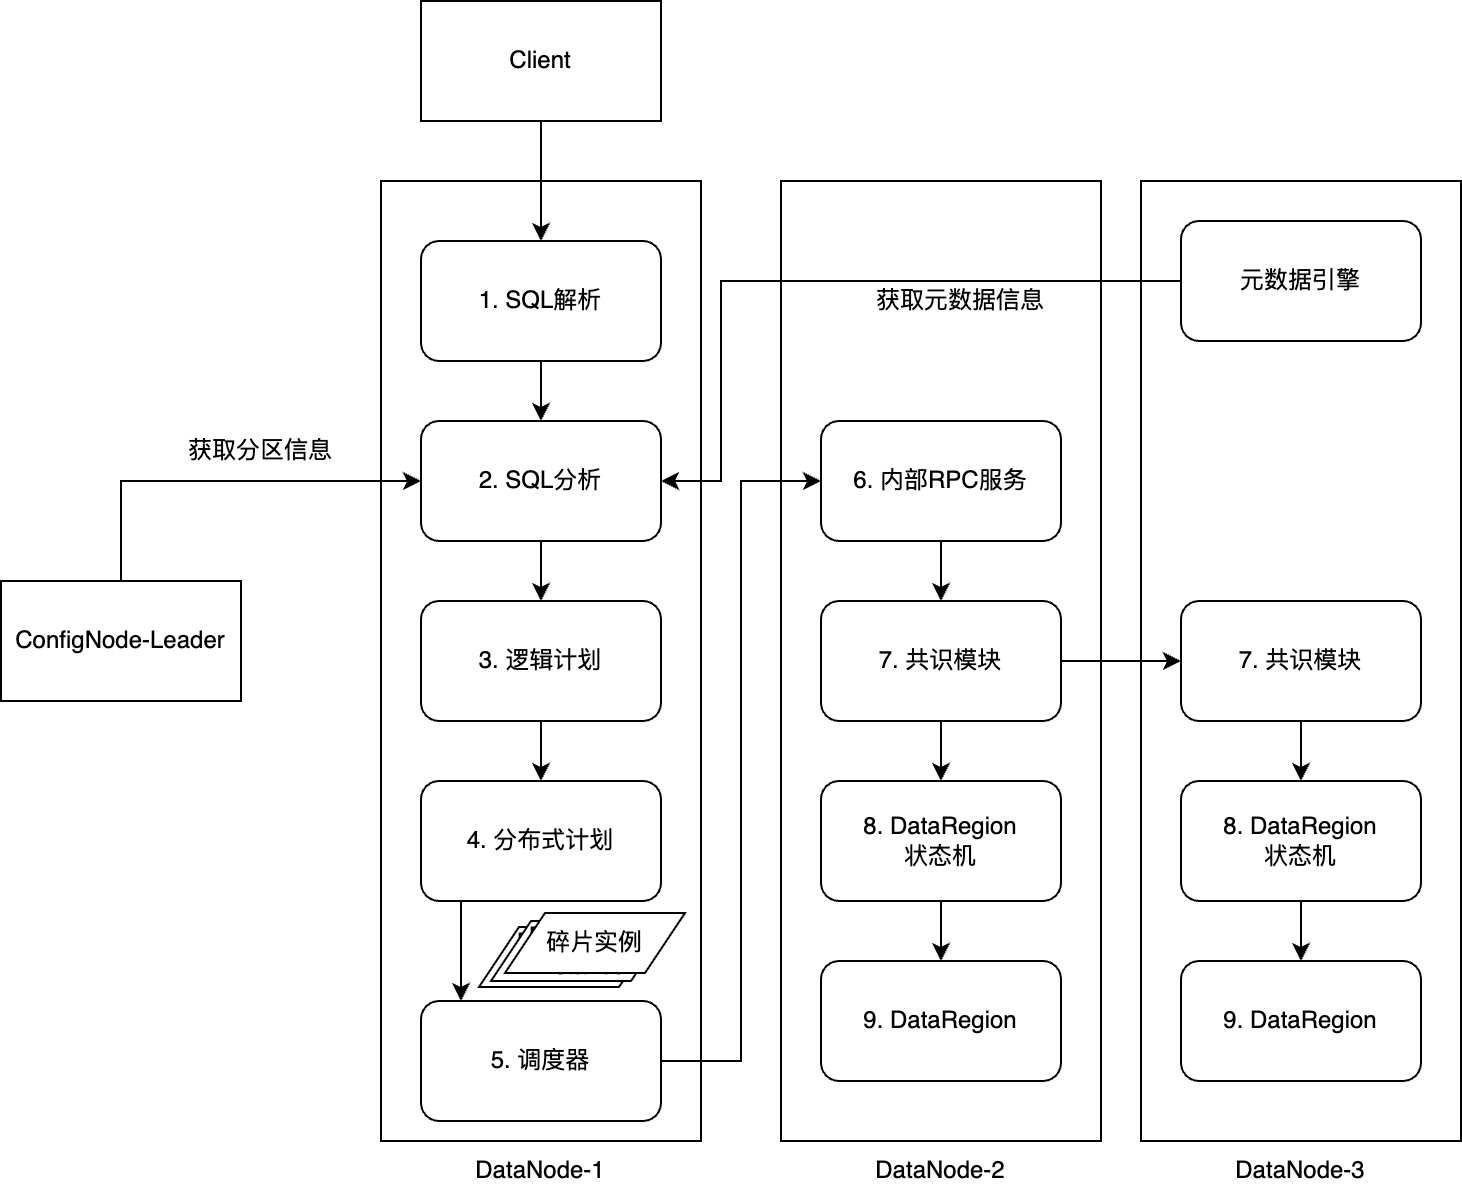
\includegraphics[width=0.99\linewidth]{c04-write-process-redraw.png}
  \caption{IoTDB写入全流程}
  \label{fig:c04-write-process}
\end{figure}

图\ref{fig:c04-write-process}展示了IoTDB现有的写入和查询流程。整个流程涉及三个主要的角色,分别是客户端的会话(Session)、数据节点的协调者(Coordinator)和共识模块的数据副本。客户端的主要作用是服务发现、连接状态管理和发送请求,Coordinator负责接受请求并进行处理,共识模块的副本则负责实际数据的写入或者读取。

第一步,客户端可以通过实例化客户端对象,和IoTDB服务端的数据节点建立连接,通过SQL等方式发起写入或者查询请求。目前,集群中的所有数据节点以连接至任意数据节点

第二步,Coordinator会对整个请求进行SQL解析(SQL Parse)。在这个阶段只进行 SQL 语法和格式的校验,确保请求在语法上的正确性。

第三步,Coordinator会进入分析(Analyze)阶段。在本阶段,Coordinator会进行权限校验,确定本次的写入或者查询要访问哪些数据,包括识别涉及的时间序列、属性以及需要查询或写入的数据范围。同时,Coordinator可能需要和管理节点 通信,获取最新的集群分区信息,了解本次访问的数据存储在哪些数据节点外,Coordinator也可能需要从其他 Data数据节点关的元数据信息。

第四步,Coordinator根据分析的结果,生成本次请求的逻辑计划。该计划描述了查询或写入操作的逻辑步骤,例如数据的选择、过滤、聚合等,但不涉及具体的物理执行方式。逻辑计划通常以逻辑查询树的形式表示。

第五步,Coordinator在逻辑计划的基础上,考虑到集群中数据的实际分布情况,数据节点该计划将逻辑操作分解为可以在不同数据节点执行的\fragmentinstance(FragmentInstance)。每个\fragmentinstance 负责处理一个特定的数据分区,具备一个副本位置集合(ReplicaSet),代表了这个分区的数据副本所在的 所有Data数据节点

第六步,Coordinator作为调度器,负责将分布式执行计划中的每个\fragmentinstance 调度到相应的数据节点上执行。对于某些操作,协调者可能会选择在本地数据节点上执行,而对于需要访问其他数据节点数据的操作,则会将相应的\fragmentinstance 发送到远程数据节点执行。如果调度过程中发生错误,协调者可能会尝试重新调度。

第七步,每一个\fragmentinstance 最终会被交付给共识层进行执行。共识层会执行相关的读写操作,并且提供数据复制和一致性的保证。以Raft共识协议为例,交给共识层的写入操作会保证被复制给大多数节点执行完成之后才会返回成功写入,交给共识层的读取操作能够保证读到线性一致性的结果。

第八步,共识模块在接收到执行指令后,会调用底层的IoTDB单机存储引擎(采用LSM架构,使用MemTable作为内存结构,使用TsFile\cite{zhao2024apachetsfile}作为持久性外部存储)进行实际的数据写入或读取操作。每个数据副本都由其所在的数据节点上的存储引擎进行管理。


\section{写入和查询请求容错原则设计}

写入和查询请求的容错原则和设计可以总结为以下几个方面:

其一,利用共识层的多副本能力进行错误转移。当某一个副本失效时,写入和查询请求应当尝试访问其他的健康副本,重试本次的请求直到成功。

其二,利用对副本的知识和集群的已知故障进行最优的执行计划规划和路由规划。如果在规划阶段,已知副本所在的节点出现了进程宕机、服务不可用、网络不可达的情况,那么在计划和规划的阶段就应该避开这些副本,绕开这些故障,从而达到最优的执行路由。

其三,一旦发现在规划、执行的阶段中由于故障的原因无法成功完成请求,那么需要尽快通知客户端节点,而不是在集群内部无意义地重试。在通知时需要尽力给出失败的原因和重试的建议,由客户端根据情况决定后续的策略。

其四,使用断措施和降级行动来防止因为重试带来的恶化。\failover 和恢复大量依赖重试的手段,然而,重试本身可能导致系统的故障更为严重。当系统故障是由于资源超配而产生时,例如负载过高导致的JVM垃圾回收时间变长、网络已经出现拥塞和超时的等情况下,频繁的重试会进一步加重集群的负担,抢占系统其他请求的存活空间,从而使系统的状态进一步恶化。为此,我们采取以下的办法:

1. 使用指数退避的重试措施。通过在重试之间引入逐渐增加的延迟,默认从100ms开始,每次重试都会翻倍。这种策略能够避免在系统短暂过载的时候引入大量的重试资源。同时,指数退避可以分散重试的时间,避免大量的失败请求因为同一个故障同时重试,导致在服务端形成一个瞬间的请求高峰。如果问题持续存在,逐渐增加的延迟会使得重试的频率降低,减少对已经处于困境的系统的持续冲击。

2. 尽量轮询每一个副本,而不是在一个副本上进行多次重试。如果某个副本本身存在问题(例如,硬件故障、配置错误等),在该副本上进行多次重试很可能仍然会失败,并且会持续消耗该副本的资源,甚至可能导致该副本彻底崩溃。轮询其他副本可以避免将所有压力集中在一个潜在的故障节点上,有助于更均匀地分配集群的负载,避免某些副本压力过大。

3. 设置最大重试次数和最大等待时间,不进行无限期重试,从而确定了一个
当达到最大重试次数后,系统会停止重试,并认为该操作最终失败。这使得系统可以及时地采取其他补救措施,例如返回错误给用户、执行降级逻辑、记录错误日志等,而不是一直停留在重试的状态。


\section{请求规划阶段的容错设计}

请求规划阶段的容错设计思路是根据集群当前的节点存活情况和副本存活情况,将\fragmentinstance 分配到最优的副本上执行。如果找不到任何一个副本来执行这个\fragmentinstance ,那么就在规划阶段就报错返回。

\subsection{基于拓扑感知的规划}\label{sec:topology-query-plan}

IoTDB协调者在进行查询规划和计划生成时,对于根节点\fragmentinstance (Root FragmentInstance)的摆放需要考虑集群的网络拓扑和分区故障。

根节点\fragmentinstance 是一种特殊的\fragmentinstance 。相较于普通的\fragmentinstance ,根节点\fragmentinstance 需要负责从其他的分布在不同的存储节点\fragmentinstance 中汇聚结果数据,进行最终数据聚合和计算,并将结果发送返回给查询的请求方。由于根节点\fragmentinstance 需要和所有的\fragmentinstance 进行通信,所以在规划期间,必须保证根节点\fragmentinstance 被调度到的节点能够和其他所有\fragmentinstance 被调度到的节点的并集联通。


\begin{figure}
  \centering
  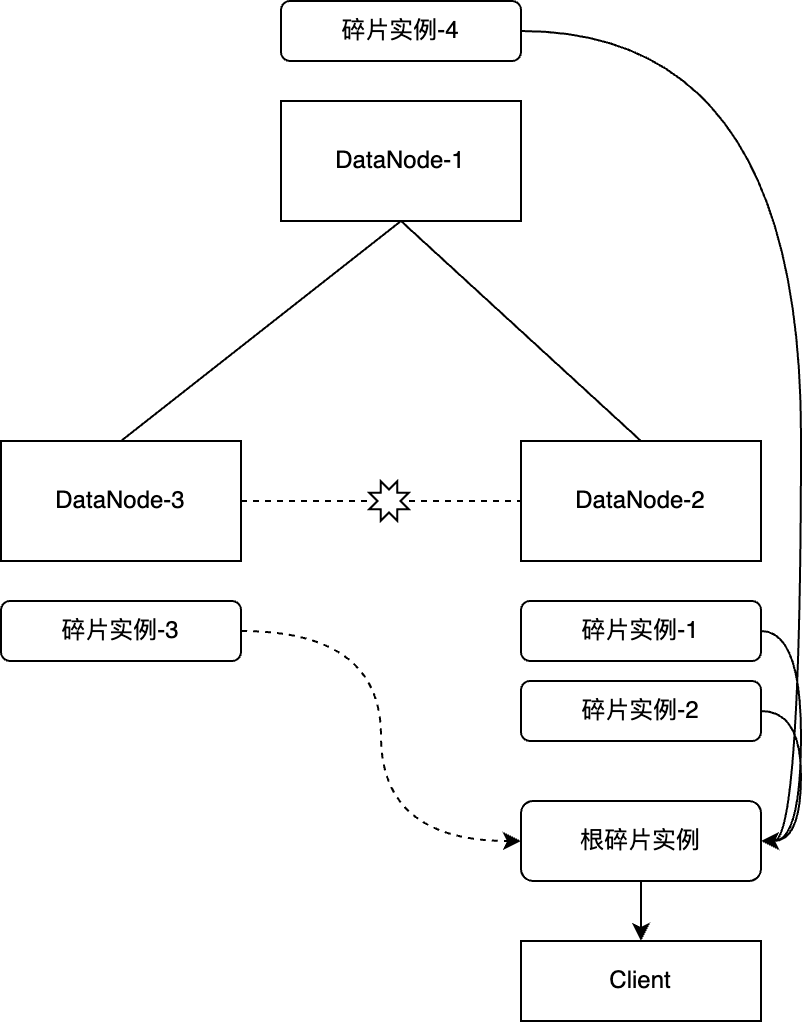
\includegraphics[width=0.6\linewidth]{c04-fi-topology-partition.redraw.png}
  \caption{网络分区下的查询失败情况}
  \label{fig:fi-topology-partition}
\end{figure}

图\ref{fig:fi-topology-partition}展示了非对称网络分区下,根节点的错误放置导致查询失败的一个例子。在这个查询中,一共有四个\fragmentinstance ,分别分布在三个数据节点上。其中第一个、第二个\fragmentinstance 被调度到了数据节点2上,第三个\fragmentinstance 被调度到了数据节点3上,第四个\fragmentinstance 被调度到了数据节点1上。

此时,数据节点2和数据节点3之间恰巧出现了非对称网络分区。如果将本次查询的根节点\fragmentinstance 调度到数据节点2上,那么这个根节点\fragmentinstance 就不能连接上第三个\fragmentinstance ,也无法收集该实例上的数据,最终导致本次查询计划失败。

因此,在决定查询计划的规划和根节点\fragmentinstance 的放置的时候,我们需要考虑节点之间的拓扑结构。根节点的\fragmentinstance 放置的数据节点必须具备和所有的\fragmentinstance 所在的数据节点都网络可达的性质。算法\ref{alg:find_candidates}给出了根节点\fragmentinstance 的放置算法。

\begin{algorithm}
  \caption{查找DataNode和FragmentInstance候选}
  \label{alg:find_candidates}
  \begin{algorithmic}
  \REQUIRE 集群拓扑结构 (连通图), FragmentInstance列表
  \ENSURE DataNode候选列表, FragmentInstance候选列表
  
  \STATE $DataNodeCandidates \leftarrow \emptyset$
  \STATE $FragmentInstanceCandidates \leftarrow \emptyset$
  
  \FOR{每个 DataNode $node$ 在 集群拓扑结构 中}
      \STATE $isCandidate \leftarrow true$
      \FOR{每个 FragmentInstance $instance$ 在 FragmentInstance列表 中}
          \STATE $foundConnection \leftarrow false$
          \FOR{每个 Replica $replica$ 在 $instance.ReplicaSet$ 中}
              \IF{$node$ 和 $replica$ 在 连通图 中连通}
                  \STATE $foundConnection \leftarrow true$
                  \STATE \textbf{break} \COMMENT{找到一个连接即可}
              \ENDIF
          \ENDFOR
          \IF{$foundConnection = false$}
              \STATE $isCandidate \leftarrow false$
              \STATE \textbf{break} \COMMENT{如果和任何ReplicaSet都无法连通,则不是候选}
          \ENDIF
      \ENDFOR
      \IF{$isCandidate = true$}
          \STATE $DataNodeCandidates \leftarrow DataNodeCandidates \cup \{node\}$
      \ENDIF
  \ENDFOR
  
  \FOR{每个 FragmentInstance $instance$ 在 FragmentInstance列表 中}
      \STATE $isCandidate \leftarrow false$
      \FOR{每个 DataNode $candidate$ 在 $DataNodeCandidates$ 中}
          \FOR{每个 Replica $replica$ 在 $instance.ReplicaSet$ 中}
              \IF{$candidate = replica$}
                  \STATE $isCandidate \leftarrow true$
                  \STATE \textbf{break} \COMMENT{找到一个候选DataNode即可}
              \ENDIF
          \ENDFOR
          \IF{$isCandidate = true$}
              \STATE \textbf{break} \COMMENT{找到一个候选DataNode即可}
          \ENDIF
      \ENDFOR
      \IF{$isCandidate = true$}
          \STATE $FragmentInstanceCandidates \leftarrow FragmentInstanceCandidates \cup \{instance\}$
      \ENDIF
  \ENDFOR
  
  \RETURN $DataNodeCandidates$, $FragmentInstanceCandidates$
  \end{algorithmic}
  \end{algorithm}

\ref{alg:find_candidates}的拓扑感知算法能够使\ref{fig:fi-topology-partition}的查询成功完成。
在该算法下,根节点\fragmentinstance 将会被调度到数据节点1节点上。由于数据节点1分别与数据节点2和数据节点3之间能够联通,因此即使出现了非对称网络分区的情况下,位于数据节点1上的根节点\fragmentinstance 依然能够成功拉取本次查询规划的所有的\fragmentinstance 的数据,成功执行查询操作。


\subsection{基于副本状态的规划}

在协调者进行查询规划时,查询规划器会从管理节点领导者获取最新的分区信息表,从而保证每一个\fragmentinstance 的副本都是最优规划的副本。该步骤包括以下的算法:

1. 规划器会首先选择主副本来执行写入和查询请求。对于RatisConsensus来说,上层应用只能选择主副本来执行写入请求。对于IoTConsensus和IoTConsensusV2来说,虽然每一个副本都能够执行写入请求,但为了避免冲突、提高系统的吞吐量,规划器依然会选择管理节点领导者指定的主副本来完成数据的写入。

2. 在主副本发生故障时,共识模块和管理节点领导者会共同保证主副本的切换。当主副本切换后,规划器就会将后续的查询请求路由到新的主副本上进行执行,从而完成\failover 和容错。在途的写入和查询请求则通过章节\ref{sec:failover-schedule}所描述的调度阶段的容错设计来实现故障的转移和容错。

3. 如果在规划时期,规划器发现某一个分区的所有副本都不可用,那么会直接使这一次查询失败,并返回失败结果给客户端,由客户端决定重试策略。

在本文的工作之前,规划器并不会使请求立即失败,而是会尝试在每一个副本之间重试,并在每一次重试中间进行一段时间的等待。这种策略常常能够解决副本组暂时性不可用的情况,但在网络分区的情况下会进行大量无谓的等待。

\begin{figure}
  \centering
  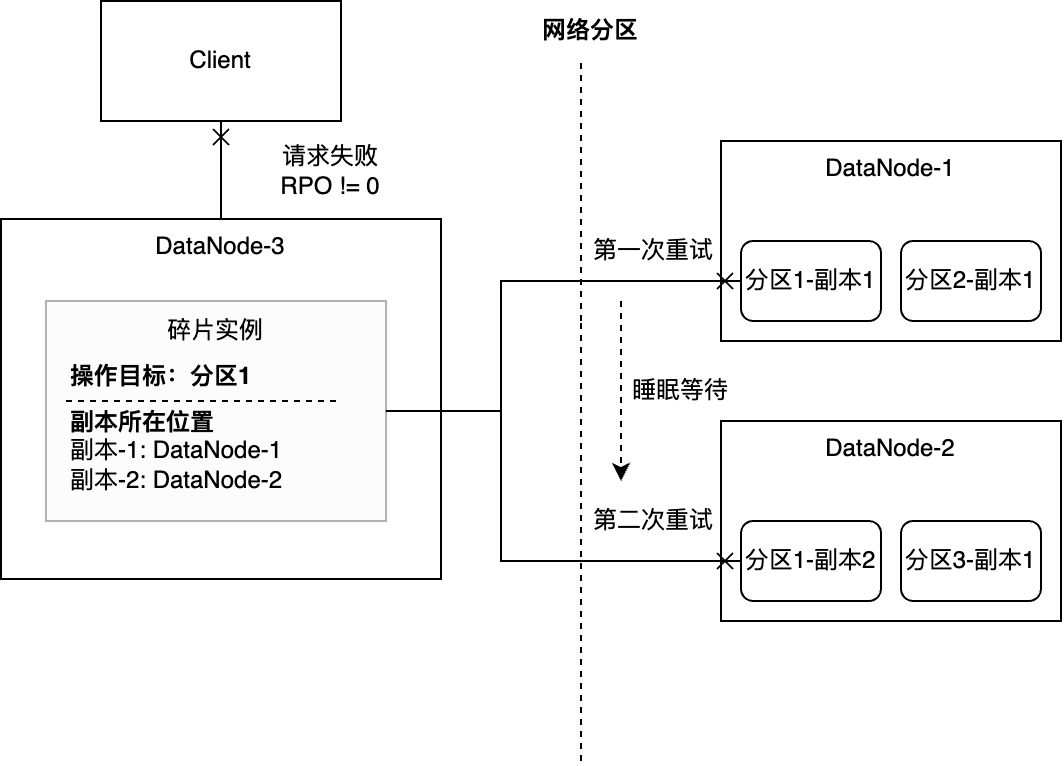
\includegraphics[width=0.9\linewidth]{c04-write-with-topology.redraw.png}
  \caption{网络分区下的写入失败情况}
  \label{fig:c04-write-with-topology}
\end{figure}

图\ref{fig:c04-write-with-topology}中展示了这种大量无谓等待的场景。
在本场景中,数据节点3与数据节点1和数据节点2之间出现了对称网络分区。此时,如果客户端连接上了数据节点3执行写入计划,该计划包含的分区的所有副本都在数据节点1和数据节点2上。
在本文之前,规划器不会立即使这次的写入失败,而是继续交给调度器。调度器会先尝试调度到数据节点1上,但是由于网络分区的问题,本次请求最终会以超时失败。接着,调度器会等待一段时间,接着尝试选择第二个副本执行,再次尝试调度,但本次请求最终依然会因为分区而失败告终。调度器会反复重复上述的重试策略,直到本次的执行超过客户端指定的超时时间,最终返回客户端失败。

这样的规划和调度存在两个问题。首先,在网络分区的情况下,客户端的请求需要经历一个完整的超时重试周期(默认为1分钟)才能被返回,这种无意义的超时和等待会严重影响客户端的吞吐。其次,如果客户端不尝试连接其他的数据节点进行重试,那么本次写入会最终失败,从而导致这部分的数据丢失,影响集群的RPO指标。

因此,本文所提出的容错设计会在发现某一个\fragmentinstance 的所有副本位置都不可达的时候,直接在规划阶段将这个请求判定为失败,返回客户端该结果,并带上建议的重试节点和方案,由客户端阶段对后续的操作做出决定。


\section{请求执行阶段的容错设计}\label{sec:failover-schedule}


请求执行阶段的容错主要面对的故障是在规划阶段未知的故障。对于规划阶段已知的故障,我们可以通过上述章节描述的最优副本选择算法进行规避。然而,如果一个副本在规划阶段尚且健康存活,但在规划结束开始执行的时候突然出现故障而无法服务请求,那么为了避免本次调度失败而导致请求失败和RPO不为零,我们需要执行阶段的容错能力。

执行阶段的容错的主要方法是对多个副本进行尝试和错误转移。
对于写请求来说,如果写入的目标副本发生了故障,本次写请求可能会出现超时无响应、返回错误码或者抛出异常,那么此时调度器需要尝试其他副本所在的数据节点进行重试,直到本次请求能够被其他的节点成功写入,或者超过配置的最大写入超时时间而返回。

对于读请求来说,情况则更为复杂,不能在副本级别进行重试,只能在请求级别进行重试。
由于根节点\fragmentinstance 需要负责从其他\fragmentinstance 中拉取数据,因此根节点在规划阶段就需要了解其他\fragmentinstance 的副本所调度的节点。如果某一个\fragmentinstance 所调度的副本出现问题,想要将重试转移到其他的副本进行调度,那么势必需要通过通知机制让根节点\fragmentinstance 了解新的调度情况和副本所在位置。这种通知机制需要极大地修改现有的查询实现和查询结构,因此在实际实现中并不可行。

为此,本文在设计读请求执行阶段的容错能力时,统一在调度错误的时候进行请求级别的重试,即重新规划这个读请求,找到最新的最优副本,然后再进行调度和执行。这种方式通过多次规划和调度的方式,能够发现在第一次规划时期未出现的错误,从而实现容错的目的。

总结来说,执行阶段的容错通过在副本级别重试、在请求级别重试的方法,对集群中那些刚刚产生但尚未被检测的故障进行容错,达到进一步提高可用性的能力。

\section{请求重试阶段的容错设计}

在请求重试阶段,客户端侧的容错设计是IoTDB集群\failover 和恢复能力的最后一块拼图,是IoTDB集群客户端与服务端协同容错的重要组成部分。

当请求经过IoTDB服务侧的重试失败返回之后,客户端可以进行最后的重试,以期通过这种方式来实现服务的可用。例如,当请求的数据节点在发生网络分区之后无法连接其他的节点,则需要发回客户端重试,让客户端连接其他的节点来完成。再例如,当集群处在变更状态中,管理节点对集群副本的状态有滞后,在规划时期出现错误规划,则需要发回客户端等待和重试,在下一次重试时,期待管理节点已经掌握了集群副本的最新状况。

此外,请求重试阶段,客户端能够自动选择最合适的数据节点完成请求。在集群正常的时期,这一功能将会把客户端的请求引导到最优节点上执行,而在集群故障的时期,这一功能将会把客户端的请求引导到能完成请求的节点上。

在正常时期,客户端虽然可以连接任何数据节点,但是为了减少在集群内部的数据转发,提高集群的整体吞吐和资源利用率,数据节点会在执行完请求之后给出一个重定向的建议。通常,被重定向的节点是客户端这些请求所需要写入的分区的主副本所在地。此时,客户端通过重定向连接到新的节点上发送请求,就能够直接在新节点上完成数据的写入,避免由其他数据节点节点进行转发。

在故障时期,例如非对称网络分区时期,数据节点的同质性被打破,并非每一个节点的都能同质地接受所有的请求。此时,为了保证集群最大的可用性,将客户端的请求尽力的完成,数据节点会在执行请求失败之后给出一个重定向和重试的建议。通常,被重定向的节点拥有更好的网络连通性,能够成功执行所有的\fragmentinstance ,从而保障了集群的可用性。

\section{本章小结}

本章聚焦于 Apache IoTDB 高可用容错框架中故障自动转移与恢复机制的设计与实现。在上一章对各类故障场景进行全面诊断的基础上,本章旨在阐述如何针对性地响应故障并引导系统恢复正常运行。

本章首先详细梳理了 IoTDB 中写入和查询请求的端到端处理流程,明确了客户端、数据节点协调者(Coordinator)以及共识模块在其中的角色与交互方式。在此基础上,提出了适用于写入和查询请求容错处理的核心设计原则,包括利用共识协议提供的多副本能力进行错误转移、基于副本状态和集群拓扑进行最优执行计划规划、快速向客户端反馈失败信息及重试建议,以及通过指数退避、副本轮询及设置最大重试次数等策略避免因重试导致的系统状态恶化。

随后,本章详细阐述了容错机制在请求处理不同阶段的设计:
在请求规划阶段,强调了基于集群当前节点存活情况和副本状态进行\fragmentinstance 分配的重要性。针对查询请求,提出了拓扑感知的规划算法,确保根节点\fragmentinstance 能够与所有相关\fragmentinstance 所在节点连通,尤其是在非对称网络分区场景下,以避免因规划失误导致的查询失败。同时,规划器能够基于副本的最新状态进行最优选择,并在检测到所有副本不可用时提前终止请求。在请求执行阶段,主要针对规划后发生的故障,通过副本级别的重试(写入请求)或请求级别的重新规划与执行(查询请求)来实现容错,确保请求不会因执行时突发的局部故障而丢失。
最后,探讨了客户端层面的请求重试容错设计,作为整个容错体系的最终保障。客户端能够依据数据节点返回的重定向建议,在正常或故障时期智能选择最优或可用的数据节点进行重试,进一步提升系统的可用性。